%%%%%%%%%%%%%%%%%%%%%%%%%%%%%%%%%%%%%%%%%
% Laboratory Report LaTeX Template
%
% This template has been downloaded from:
% http://www.latextemplates.com
%
% Original header:
%
% This is a LaTeX version of the sample laboratory report
% from Virginia Tech's copyrighted 08-09 CHEM 1045/1046 lab manual.
% Reproduction of this one appendix section for academic purposes
% should fall under fair use.
%
%%%%%%%%%%%%%%%%%%%%%%%%%%%%%%%%%%%%%%%%%

%----------------------------------------------------------------------------------------
%	DOCUMENT CONFIGURATIONS
%----------------------------------------------------------------------------------------

\documentclass{article}

\title{Practical 1\\ Aurora Borealis} % Title

\def\authors{
Ivan \v Sinkarenko\\
Anuraj Rajendraprakash
}
\author{\authors}
%\author{Ivan \textsc{Sinkarenko}} % Author name
%\author{Anuraj \textsc{Rajendraprakash}} % Author name

\usepackage{graphicx}
\begin{document}

\maketitle % Insert the title, author and date

\centerline{Referee: Dr. Gabriella Stenberg}

\setlength\parindent{0pt} % Removes all indentation from paragraphs

\renewcommand{\labelenumi}{\alph{enumi}.} % Make numbering in the enumerate environment by letter rather than number (e.g. section 6)

%----------------------------------------------------------------------------------------
%	SECTION 1. Objectives
%----------------------------------------------------------------------------------------

\section{Objectives}

\textbf{TBD}

% If you have more than one objective, uncomment the below:
%\begin{description}
%\item[First Objective] \hfill \\
%Objective 1 text
%\item[Second Objective] \hfill \\
%Objective 2 text
%\end{description}
 
%----------------------------------------------------------------------------------------
%	SECTION 2. Classification
%----------------------------------------------------------------------------------------

\section{Classification}

\textbf{TBD}

%----------------------------------------------------------------------------------------
%	SECTION 3. Auroral Forecast
%----------------------------------------------------------------------------------------

\section{Auroral Forecast}

The purpose of this part of the assignment is to analyse data from different sensors and predict whether it is suitable conditions for seeing Aurora Borealis or not. However, by the time this report has been written (April 26, 2012) it was not possible to see the northern lights because it didn't get dark enough during the night time. For this reason, this section contains the analysis of the data taken from previous month and is compared to the images from the Auroral Large Imaging System (ALIS).
\\
The data for analysis was taken from May 28, 2012 because it was quite a spectacular Aurora that day. As a source of images and scientific data the website of Swedish Institude of Space Physics (IRF) was used. The scientific data implies magnetometer and riometer measurements.

\subsection{Magnetometer}
Magnetometer is often used to measure long- and short-term variations. The Kiruna flux-gate magnetometers are used to measure short-term variations, which are due to electric currents flowing in the ionosphere and induced in the surface layers in the solid Earth. The time resolution for the data measurement of these particular sensors is 20 seconds. The key properties of the magnetic disturbance level are:

\begin{itemize}
\item K-indices: Quasi-logarithmic scale from 0 (very quiet) through 3 (moderately disturbed) to 9 (very disturbed).
\item $A_p$ index: A linear, daily index ranging from 0 (very quiet) through 15 (moderately disturbed) to 400 (very disturbed).
\item $A_E$ index: Index of auroral activity, derived from horizontal component of magnetic field variation at 10-12 auroral-zone observatories.
\item $D_{st}$ index: Index of ring-current (and global magnetic storms), derived from near equator observatories.
\end{itemize}

The flux-gate data from Kiruna's magnetometers is calibrated against the absolute measurments each month. Afterwards, quiet days are identified and the K-indices are calculated. In the geomagnetic measurements disturbance variations might be a sign of an aurora.

\subsection{Riometer}
The Relative Ionosphere Opacity meters (riometers) are used to measure the absorbtion of radio-noise from the starts in the ionosphere and they operate at 25-50 Mhz frequency. Radio waves of this frequency are absorbed at the altitude of 60-110 km if there is a significant number of electrons present in ionosphere.

Riometers perform continuous observations of the noise-level and observe decreases in noise relative to the quite-day level when there is increased ionization due to the precipitation of the high energy electrons and protons. The typical auroral signature on the riogram is a sharp dip of few dB, followed by the slow regrowth. IRF has two riometers working at 30 and 38 MHz.

\subsection{Analysis}
The measurements taken from the archive for 28th of March are show in the figures below, where Figure \ref{fig:magnetometer} represents magnetometer measurements and Figure \ref{fig:riometer} represents riogram.

\begin{figure}[htbp!]
\centering
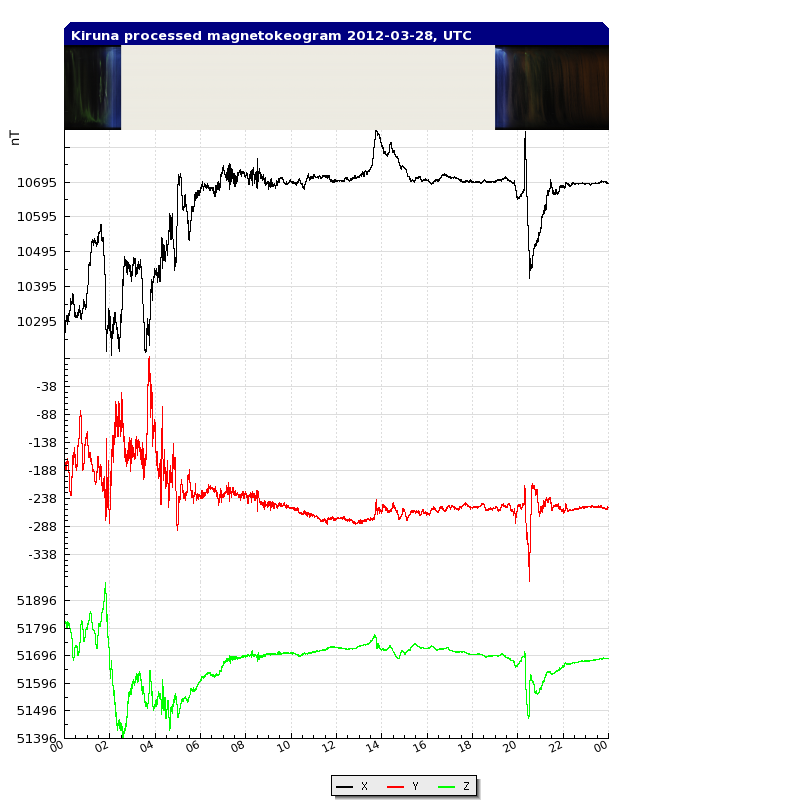
\includegraphics[width=1.3\textwidth]{Figures/magnetometer.png}
\caption{Magnetogram for the 28th of March, 2012.}
\label{fig:magnetometer}
\end{figure}

\begin{figure}[htbp!]
\centering
\centerline{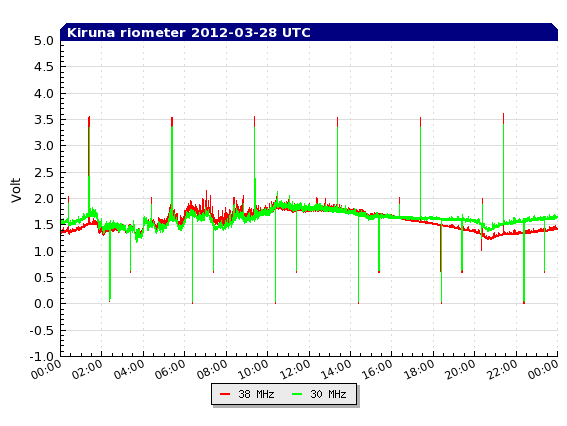
\includegraphics[width=1\textwidth]{Figures/riometer.png}}
\caption{Riogram for the 28th of March, 2012.}
\label{fig:riometer}
\end{figure}

As it is seen in the magnetogram, there we quite some fluctuations from 00:00 to 08:00 at night of 28th of March. However, images are not recorded though the entire night because at the certain point it becomes to bright to see the aurora. Riometer has also some fluctuations during that time. Therefore, we can assume that there were a high probability of auroral display. However, to make sure that our assumptions are correct we decided to focus on the disturbances, occurred in the period from 20:00 to 22:00. The magnetometer clearly shows the variations in the magnetic field and the riometer has a dip, followed by the ramp of magnetic field recovery. Based on this observations, we conclude that there should have been a strong aurora during that period.

To check if the predictions were correct or not the pictures from the archive were taken for the period we are interested in. Compilation of 12 images from ALIS is shown in Figure \ref{fig:ALIS}. According to the datagrams the auroral peak was around 21:00. On the ALIS images, the one taken at 20:51 is the brightest which is approximately at the same time as expected. To sum up, it is seen that the measurements reflect the real auroral probability correctly.

\begin{figure}[htbp!]
\centering|
\centerline{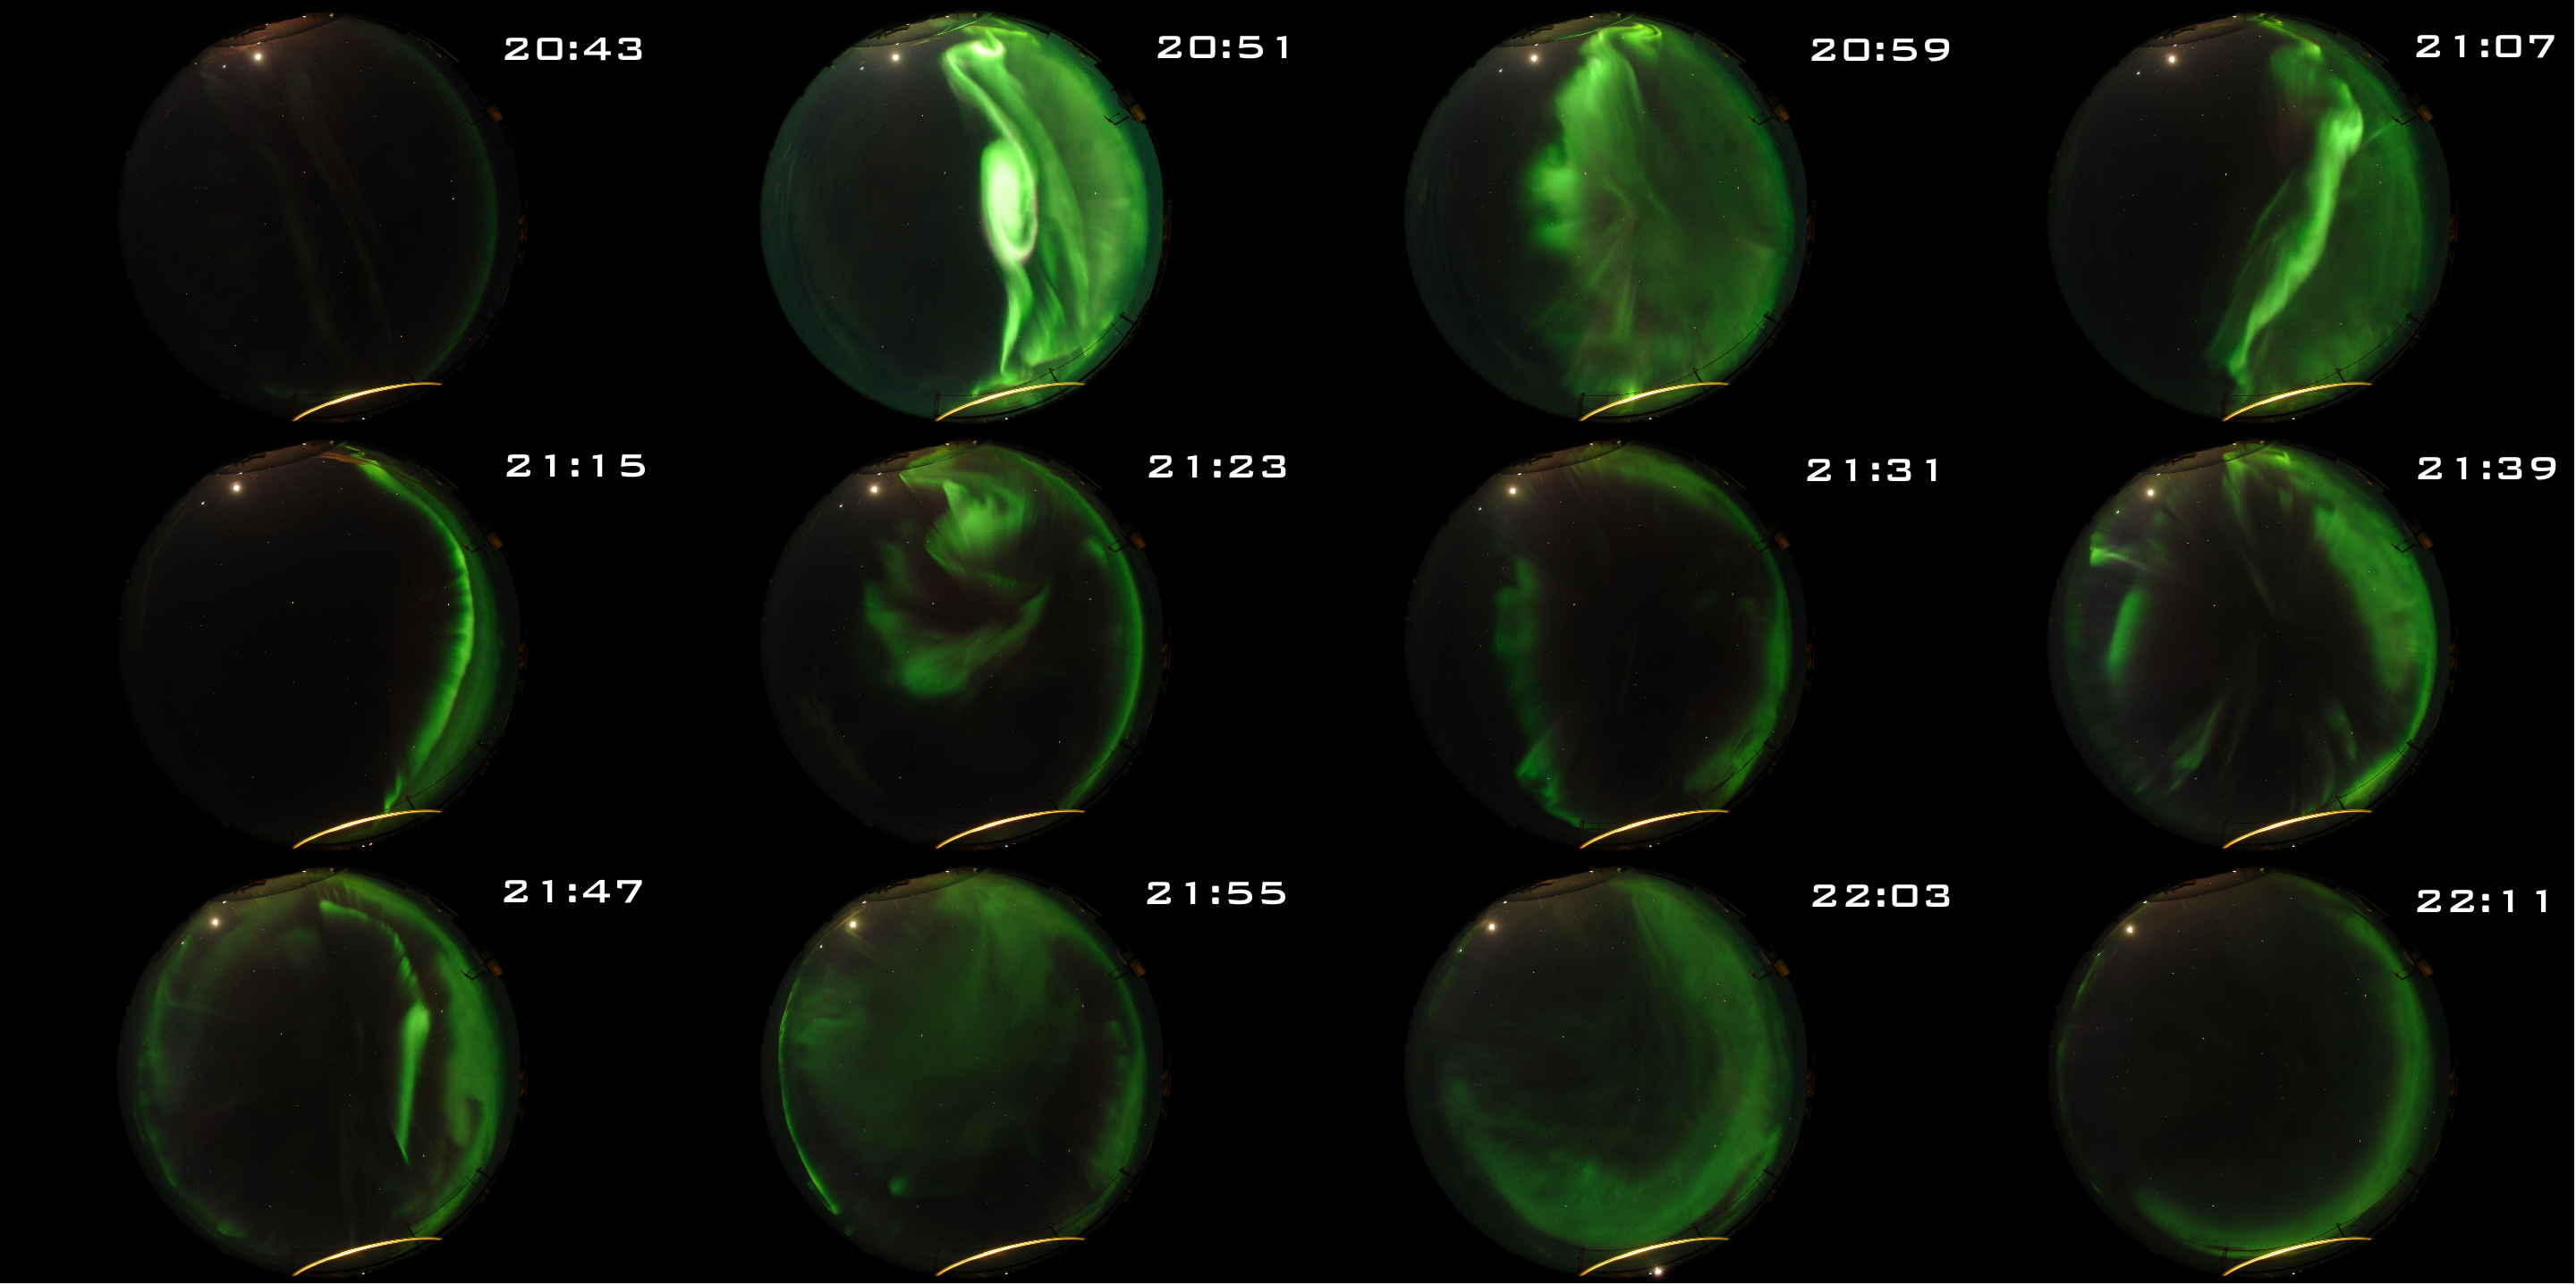
\includegraphics[width=1.5\textwidth]{Figures/awowa.png}}
\caption{ALIS images compilation between 20:30 and 22:30 of March 28, 2012. The time in the upper right corner of each single picture represent the time it was taken.}
\label{fig:ALIS}
\end{figure}


%----------------------------------------------------------------------------------------
%	SECTION 4. Results and Conclusions
%----------------------------------------------------------------------------------------

\section{Results and Conclusions}

\textbf{TBD for the first part}
\\
The date of the environment was chosen based on personal observations. During the experiment, datagrams from the magnetometer and riometer were compared to the images taken by ALIS. All the data was fetched from the IRF archives. The analysis showed that the highest probability of the aurora took place at the same time as there was the brightest aurora according to the images. As a result, we conclude that we have understood the principle how the predictions are made based on the data analysis and what processes are responsible for studied behavior.

%----------------------------------------------------------------------------------------
%	BIBLIOGRAPHY
%----------------------------------------------------------------------------------------

\begin{thebibliography}{9}

\bibitem{Stenberg:2012ab}
Stenberg, G.  (2012).
\newblock {\em Practical 1. Aurora Borealis}.
\newblock Swedish Institute of Space Physics, Kiruna, Sweden.

\bibitem{KivelsonRussell:1996isp}
Kivelson M. ~G. and Russell C. ~T.  (1996).
\newblock {\em Introduction to Space Physics}.
\newblock Cambridge University Press, Melbourne, Australia.

\end{thebibliography}

\end{document}